\documentclass[10pt,a4paper]{article}

\usepackage[a4paper,top=18mm,bottom=19mm,left=18mm,right=18mm,headsep=7mm,footskip=9mm]{geometry}
\usepackage{fontspec}
\setsansfont{TeX Gyre Heros}
\setmainfont{TeX Gyre Heros}
\renewcommand{\familydefault}{\sfdefault}
\usepackage{microtype}
\usepackage{xcolor}
\usepackage{graphicx}
\usepackage{booktabs}
\usepackage{array}
\usepackage{tabularx}
\usepackage{tikz}
\usetikzlibrary{arrows.meta,positioning,calc,shapes.geometric}
\usepackage{hyperref}
\usepackage{fancyhdr}
\usepackage{caption}
\usepackage{float}
\usepackage{ragged2e}

\definecolor{Navy}{HTML}{0B132B}
\definecolor{Ink}{HTML}{172033}
\definecolor{Muted}{HTML}{667085}
\definecolor{Line}{HTML}{DDE3EC}
\definecolor{Soft}{HTML}{F5F7FB}
\definecolor{Cyan}{HTML}{00A6C8}
\definecolor{CyanSoft}{HTML}{EAF9FC}
\definecolor{Violet}{HTML}{7C5CFC}
\definecolor{VioletSoft}{HTML}{F1EEFF}
\definecolor{Green}{HTML}{12A676}
\definecolor{GreenSoft}{HTML}{EAF8F3}
\definecolor{Amber}{HTML}{F29D38}
\definecolor{AmberSoft}{HTML}{FFF5E8}
\definecolor{Rose}{HTML}{E2556F}
\definecolor{RoseSoft}{HTML}{FFF0F3}

\hypersetup{colorlinks=true,linkcolor=Cyan,urlcolor=Cyan,citecolor=Cyan,pdfauthor={HelioSat},pdftitle={Validación del pronóstico de tormentas geomagnéticas}}
\setlength{\parindent}{0pt}
\setlength{\parskip}{5pt}
\setlength{\headheight}{19pt}
\setlength{\emergencystretch}{2em}
\renewcommand{\arraystretch}{1.22}
\let\plainsection\section
\renewcommand{\section}[1]{\plainsection{\color{Navy}#1}}
\let\plainsubsection\subsection
\renewcommand{\subsection}[1]{\plainsubsection{\color{Ink}#1}}

\pagestyle{fancy}
\fancyhf{}
\fancyhead[L]{\footnotesize\color{Muted}\textbf{HELIOSAT} / Validación geomagnética}
\fancyhead[R]{\footnotesize\color{Muted}Informe divulgativo / Agosto 2026}
\fancyfoot[L]{\scriptsize\color{Muted}Candidato retrospectivo. No representa todavía un SLA operacional.}
\fancyfoot[R]{\scriptsize\color{Muted}\thepage}
\renewcommand{\headrulewidth}{0.4pt}
\renewcommand{\headrule}{\hbox to\headwidth{\color{Line}\leaders\hrule height \headrulewidth\hfill}}

\newsavebox{\summarysave}
\newsavebox{\warningsave}
\newsavebox{\resultsave}
\newenvironment{summarybox}{\begin{center}\setlength{\fboxsep}{4mm}\begin{lrbox}{\summarysave}\begin{minipage}{0.90\textwidth}}{\end{minipage}\end{lrbox}\colorbox{CyanSoft}{\usebox{\summarysave}}\end{center}}
\newenvironment{warningbox}{\begin{center}\setlength{\fboxsep}{4mm}\begin{lrbox}{\warningsave}\begin{minipage}{0.90\textwidth}}{\end{minipage}\end{lrbox}\colorbox{AmberSoft}{\usebox{\warningsave}}\end{center}}
\newenvironment{resultbox}{\begin{center}\setlength{\fboxsep}{3mm}\begin{lrbox}{\resultsave}\begin{minipage}{0.91\textwidth}}{\end{minipage}\end{lrbox}\fcolorbox{Line}{white}{\usebox{\resultsave}}\end{center}}
\newcommand{\metric}[3]{\begin{minipage}[t]{0.30\linewidth}\centering{\scriptsize\color{Muted}\MakeUppercase{#1}}\\[2pt]{\fontsize{20}{22}\selectfont\bfseries\color{#3}#2}\end{minipage}}
\newcommand{\source}[1]{\textsuperscript{\color{Cyan}\textbf{[#1]}}}
\pdfstringdefDisableCommands{\def\color#1{}}

\begin{document}

\hypersetup{pageanchor=false}
\begin{titlepage}
\begin{tikzpicture}[remember picture,overlay]
  \fill[Navy] (current page.south west) rectangle (current page.north east);
  \fill[Cyan] (current page.north west) rectangle ([xshift=8mm]current page.south west);
  \fill[Cyan,opacity=0.13] ([xshift=-15mm,yshift=-24mm]current page.north east) circle (44mm);
  \fill[Violet,opacity=0.15] ([xshift=-5mm,yshift=18mm]current page.south east) circle (58mm);
  \draw[Cyan,opacity=0.28,line width=0.5pt] ([xshift=-92mm,yshift=-37mm]current page.north east) circle (27mm);
  \draw[Cyan,opacity=0.18,line width=0.5pt] ([xshift=-92mm,yshift=-37mm]current page.north east) circle (37mm);
\end{tikzpicture}
\color{white}
\vspace*{12mm}
{\small\bfseries\color{Cyan}HELIOSAT / VALIDATION \& STUDIES}\par
\vspace{32mm}
{\fontsize{30}{34}\selectfont\bfseries Pronóstico de tormentas\\geomagnéticas}\par
\vspace{7mm}
{\Large\color{white!78}Cómo lo medimos, qué aprende el modelo\\y qué significan realmente los resultados}\par
\vspace{14mm}
\colorbox{Navy!75!white}{\parbox{0.72\textwidth}{\color{white}\small\vspace{2mm}Un informe técnico escrito para poder leerse sin conocimientos previos de física espacial ni de machine learning. El foco está en las preguntas prácticas: qué datos entran, cuánto avisa el sistema y cuántas tormentas detecta, pierde o alerta por error.\vspace{2mm}}}
\vfill
\begin{tabular}{@{}ll@{}}
\color{white!55}\small Periodo de datos & \color{white}\small 1995 - abril de 2026\\
\color{white!55}\small Test final & \color{white}\small 2024 - abril de 2026\\
\color{white!55}\small Objetivo cliente & \color{white}\small Tormentas G3 y superiores\\
\color{white!55}\small Estado & \color{white}\small Candidato retrospectivo / todavía no live\\
\end{tabular}
\vspace{11mm}
{\footnotesize\color{white!50}Versión 1.0 / Agosto de 2026}
\end{titlepage}
\hypersetup{pageanchor=true}
\pagenumbering{arabic}

\section{La historia en un minuto}

El modelo observa el viento solar antes de que llegue a la Tierra. A partir de su velocidad, densidad y campo magnético estima cómo de fuerte será la respuesta geomagnética. Esa respuesta se expresa como Kp y, para clientes, como nivel G1, G2, G3, G4 o G5.

La idea es sencilla: si medimos una estructura peligrosa aguas arriba, cerca del punto L1, podemos avisar mientras viaja hacia la Tierra. En el test final, el tiempo de tránsito calculado tiene una mediana de \textbf{51 minutos}. Es la antelación de la parcela solar observada, no una promesa exacta sobre el minuto de inicio de Kp.

\begin{summarybox}
\textbf{Resultado principal.} En datos nunca utilizados para entrenar, desde enero de 2024 hasta abril de 2026, HelioSat identificó \textbf{16 de 27 episodios G3+}. Emitió cuatro falsas alarmas G3+ y perdió once tormentas. La precisión fue del \textbf{80,0\%} y el recall del \textbf{59,3\%}.
\end{summarybox}

\vspace{3mm}
\begin{resultbox}
\centering
\metric{Precisión G3+}{80,0\%}{Green}\hfill
\metric{Recall G3+}{59,3\%}{Cyan}\hfill
\metric{Error medio Kp}{0,44}{Violet}
\end{resultbox}

Estos números son claramente mejores que los de la heurística anterior, pero todavía no justifican un SLA comercial. El motivo es estadístico: 27 tormentas severas siguen siendo pocas y generan intervalos de confianza amplios. El resultado debe leerse como \textbf{evidencia prometedora para un despliegue en shadow mode}, no como una garantía operacional.

\section{Qué se observa, dónde y con qué fuente}

No hay una única misión que haga todo el recorrido. Cada tramo utiliza una fuente distinta y tiene un papel muy concreto.

\begin{center}
\begin{tikzpicture}[node distance=8mm and 7mm,>=Latex]
\tikzset{flowbox/.style={rounded corners=2mm,minimum width=37mm,minimum height=24mm,align=center,draw=Line,fill=white,text=Ink,font=\small}, arrow/.style={->,thick,Cyan}}
\node[flowbox,fill=CyanSoft] (l1) {\textbf{1. Viento solar}\\[-1pt]\scriptsize Wind, ACE, IMP 8, Geotail\\\scriptsize vía NASA OMNI};
\node[flowbox,right=of l1,fill=VioletSoft] (prop) {\textbf{2. Propagación}\\[-1pt]\scriptsize geometría MRU HelioSat\\\scriptsize L1 hacia la Tierra};
\node[flowbox,right=of prop,fill=GreenSoft] (kp) {\textbf{3. Respuesta real}\\[-1pt]\scriptsize 13 observatorios terrestres\\\scriptsize Kp definitivo GFZ};
\node[flowbox,right=of kp,fill=AmberSoft] (score) {\textbf{4. Evaluación}\\[-1pt]\scriptsize alertas, aciertos, errores\\\scriptsize y tiempo de aviso};
\draw[arrow] (l1) -- (prop);
\draw[arrow] (prop) -- (kp);
\draw[arrow] (kp) -- (score);
\end{tikzpicture}
\end{center}

\subsection{Tramo 1: las medidas aguas arriba}

La entrada procede de \textbf{High Resolution OMNI}, un producto armonizado por NASA/SPDF con resolución de cinco minutos. OMNI no es una misión: intercala medidas de las misiones \textbf{Wind, ACE, IMP 8 y Geotail}, conserva la procedencia y desplaza temporalmente los registros hacia una referencia próxima al bow shock.\source{1}

De cada registro se utilizan velocidad del viento solar, componentes del campo magnético IMF, densidad, presión, temperatura y posición de la nave. A partir de ellos se construyen 59 variables físicas, entre ellas campo sur, presión dinámica, acoplamiento de Newell, epsilon y memoria de las tres a nueve horas anteriores.

\subsection{Tramo 2: de L1 a la Tierra}

HelioSat reconstruye cuándo estaba disponible cada medida en L1 y vuelve a calcular su llegada con una propagación MRU. El Timeshift retrospectivo de OMNI se usa para recuperar el instante de observación, pero no entra como predictor. Esta decisión reduce fugas temporales, aunque no elimina la necesidad de una validación futura con el feed live real.

\subsection{Tramo 3: qué ocurrió realmente}

La referencia final es el \textbf{Kp planetario definitivo de GFZ}. No procede de un satélite, sino de 13 observatorios geomagnéticos distribuidos por el planeta. GFZ publica una estimación provisional o nowcast y, más tarde, el valor definitivo utilizado en este estudio.\source{2}

\begin{warningbox}
\textbf{Una limitación importante del estándar actual.} El Kp oficial tiene una resolución de \textbf{tres horas}. Aunque HelioSat use entradas cada cinco minutos, no existe una etiqueta Kp definitiva por minuto. Kp puede difuminar el instante de inicio y los picos dentro de cada intervalo. Es una limitación estructural del índice incumbente, no una decisión de muestreo de HelioSat.
\end{warningbox}

\section{Qué aprende el modelo y qué dejamos para evaluar}

Separar entrenamiento y evaluación es esencial. Si el modelo ve durante su desarrollo los mismos eventos con los que luego se puntúa, el resultado puede parecer mejor de lo que realmente es.

\begin{table}[H]
\centering
\caption*{Separación cronológica utilizada}
\begin{tabularx}{\textwidth}{>{\bfseries}p{31mm}p{34mm}Xr}
\toprule
Bloque & Fechas & Para qué se utiliza & Tamaño\\
\midrule
Desarrollo & 1995 - 2023 & Entrenar, seleccionar complejidad y fijar umbrales mediante validación cronológica & 71.718 bins\\
Test final & 2024 - abril 2026 & Abrir una sola vez y medir el resultado final & 6.465 bins\\
\bottomrule
\end{tabularx}
\end{table}

En total se procesaron \textbf{2.933.254 registros de cinco minutos}. El desarrollo contiene 922 episodios G1+ y 90 G3+. El test final contiene 131 episodios G1+ y 27 G3+.

No se amplía artificialmente el test hacia atrás para conseguir una cifra más atractiva. Empezar en 2021 solo aportaría seis eventos G3+ adicionales y esos años ya participaron en la selección del modelo. En su lugar mostramos dos capas de evidencia, con resultados separados: 68 eventos G3+ de validación histórica y 27 del test final.

\begin{figure}[H]
\centering

\includegraphics[width=0.92\textwidth]{figures/evidence-split.pdf}
\caption{La validación histórica aporta contexto y el test final conserva la independencia. No se mezclan ambos scores en una única cifra.}
\end{figure}

\section{Cuatro productos parecidos, pero no equivalentes}

NOAA forecast, HelioSat y GFZ nowcast publican números con aspecto de Kp, pero responden a preguntas distintas. Compararlos sin mostrar la antelación llevaría a una conclusión equivocada.

\begin{table}[H]
\centering
\small
\begin{tabularx}{\textwidth}{>{\bfseries}p{30mm}p{24mm}p{31mm}X}
\toprule
Producto & Tipo & Antelación & Lectura correcta\\
\midrule
NOAA next day & Pronóstico & 23,5 - 44,5 h & Mucha antelación; todavía no ha observado en L1 la estructura que llegará al día siguiente.\\
NOAA two day & Pronóstico & 47,5 - 68,5 h & Horizonte aún más difícil; ofrece contexto estratégico, no una alarma de última hora.\\
HelioSat & Pronóstico & Mediana 47 min & Ya observa la parcela en L1 y estima su llegada e impacto. Menos horizonte, más información física directa.\\
GFZ nowcast & Nowcast & Sin antelación positiva & Estima la respuesta geomagnética que ya está ocurriendo o acaba de ocurrir. Es una referencia, no un competidor predictivo.\\
GFZ definitive & Observación final & Retrospectivo & Es la verdad utilizada para puntuar a todos los demás.\\
\bottomrule
\end{tabularx}
\end{table}

Para que la comparación sea justa se usan exactamente los mismos \textbf{3.694 intervalos}, desde el 3 de enero de 2025 hasta el 30 de abril de 2026. Se conserva una sola emisión NOAA diaria, la de las 00:30 UTC. En este subconjunto común ocurrieron 90 episodios G1+ y 14 G3+.

\begin{figure}[H]
\centering

\includegraphics[width=\textwidth]{figures/product-comparison.pdf}
\caption{Precisión y recall a nivel de evento. El buen resultado de GFZ nowcast debe interpretarse junto con su ausencia de antelación. La comparación G3+ contiene solo 14 eventos y, por ello, tiene alta incertidumbre.}
\end{figure}

La lectura práctica es la siguiente:
\begin{itemize}
  \item \textbf{NOAA ofrece tiempo para prepararse}, pero su recall es bajo en este archivo cuando exigimos acertar el episodio Kp exacto.
  \item \textbf{HelioSat ofrece menos tiempo}, alrededor de 47 minutos en el subconjunto común, pero detecta una fracción mucho mayor de los episodios porque ya ha medido la estructura solar en L1.
  \item \textbf{GFZ nowcast es el más parecido al definitivo}, como cabría esperar: está describiendo una respuesta terrestre ya presente y no anticipándola.
\end{itemize}

\begin{warningbox}
Esta figura no demuestra que HelioSat sea ``mejor que NOAA'' de forma general. Demuestra que resuelve una tarea diferente: NOAA intenta mirar uno o dos días hacia delante; HelioSat hace una alerta física de corto plazo cuando la perturbación ya ha llegado a L1.
\end{warningbox}

\section{Aciertos, falsas alarmas y tormentas perdidas}

Para hablar con claridad, agrupamos los intervalos Kp consecutivos en episodios. Una tormenta de nueve horas no cuenta como tres casos independientes. Una alerta y una tormenta se consideran emparejadas si se solapan con una tolerancia predefinida de un bin Kp, es decir, tres horas.

\begin{table}[H]
\centering
\begin{tabularx}{\textwidth}{>{\bfseries\raggedright\arraybackslash}p{32mm}>{\raggedright\arraybackslash}p{48mm}>{\raggedright\arraybackslash}X}
\toprule
Concepto & Qué ocurrió & Traducción natural\\
\midrule
True positive (TP) & Alertamos y hubo tormenta & Un acierto\\
False positive (FP) & Alertamos y no hubo tormenta emparejada & Una falsa alarma\\
False negative (FN) & No alertamos y sí hubo tormenta & Una tormenta perdida\\
True negative (TN) & No alertamos y no hubo tormenta & Un periodo tranquilo correctamente ignorado\\
\bottomrule
\end{tabularx}
\end{table}

\textbf{Precisión} pregunta: ``cuando alertamos, ¿cuántas veces teníamos razón?''. Se calcula como $TP/(TP+FP)$. \textbf{Recall} pregunta: ``de todas las tormentas reales, ¿cuántas encontramos?''. Se calcula como $TP/(TP+FN)$.

\begin{figure}[H]
\centering

\includegraphics[width=\textwidth]{figures/event-outcomes.pdf}
\caption{Resultados del candidato HelioSat en el test final 2024 - abril 2026.}
\end{figure}

\begin{table}[H]
\centering
\small
\caption*{Resumen a nivel de episodio}
\begin{tabular}{lrrrrrr}
\toprule
Umbral & Eventos reales & TP & FP & FN & Precisión & Recall\\
\midrule
G1+ / Kp $\geq 5$ & 131 & 94 & 66 & 37 & 58,8\% & 71,8\%\\
G3+ / Kp $\geq 7$ & 27 & 16 & 4 & 11 & 80,0\% & 59,3\%\\
\bottomrule
\end{tabular}
\end{table}

Para G3+, ocho de cada diez alertas fueron correctas, pero el sistema encontró aproximadamente seis de cada diez tormentas reales. La precisión es buena; el principal margen de mejora está en reducir las once tormentas severas perdidas. El umbral operacional deberá elegirse según el coste real de una falsa alarma frente al coste de no avisar una G3+.

\section{Qué cambió al entrenar de verdad}

La versión anterior era una regla física fija basada principalmente en velocidad y campo magnético sur. Era interpretable, pero no aprendía de los casos históricos. El nuevo candidato combina 59 variables y ajusta por separado las probabilidades de G1+ y G3+, además de producir una estimación continua de Kp.

\begin{figure}[H]
\centering

\includegraphics[width=0.76\textwidth]{figures/baseline-improvement.pdf}
\caption{Comparación G3+ sobre el mismo test final. CSI resume aciertos, falsas alarmas y eventos perdidos en una sola métrica.}
\end{figure}

\begin{center}
\begin{tabular}{lrr}
\toprule
Métrica continua & Heurística anterior & Modelo entrenado\\
\midrule
Error absoluto medio Kp & 0,92 & \textbf{0,44}\\
RMSE Kp & 1,13 & \textbf{0,57}\\
Correlación con Kp definitivo & 0,754 & \textbf{0,918}\\
Sesgo medio Kp & +0,63 & \textbf{+0,05}\\
\bottomrule
\end{tabular}
\end{center}

La mejora no consiste solo en acercarse más al valor Kp. Para G3+, el modelo pasa de 11 a 16 tormentas detectadas y reduce las falsas alarmas de cinco a cuatro. El recall sube de 40,7\% a 59,3\%, mientras que la precisión aumenta de 68,8\% a 80,0\%.

\section{Un ejemplo: la tormenta de mayo de 2024}

La tormenta de mayo de 2024 es un buen ejemplo porque pertenece por completo al test final. El modelo no utilizó ese episodio durante el entrenamiento ni para elegir sus umbrales.

\begin{figure}[H]
\centering

\includegraphics[width=\textwidth]{figures/may-2024-episode.pdf}
\caption{Evolución del Kp definitivo, la estimación del candidato y la heurística anterior. Cada punto sigue representando un intervalo Kp oficial de tres horas.}
\end{figure}

El candidato sigue bien la subida principal y reproduce la fase severa mucho mejor que la regla anterior. Aun así, el gráfico también enseña por qué no debemos reducir toda la validación a un caso espectacular: el resultado comercial se decide con las 27 tormentas G3+ del test, incluidas las once que no detectó.

\section{Qué podemos afirmar y qué falta}

\begin{summarybox}
\textbf{Afirmación razonable hoy.} El candidato entrenado mejora materialmente la heurística anterior y produce una señal de corto plazo útil para tormentas severas. En el test final obtuvo 80,0\% de precisión G3+ y 59,3\% de recall G3+, con una mediana de 51 minutos de tránsito L1 - Tierra.
\end{summarybox}

\textbf{Todavía no deberíamos afirmar} que la precisión live será exactamente la misma, que existe un SLA de 51 minutos o que HelioSat sustituye el pronóstico de uno o dos días de NOAA. Hay tres razones:
\begin{itemize}
  \item El test contiene solo 27 episodios G3+; el intervalo de confianza del recall es 40,7\% - 75,5\%.
  \item OMNI utiliza un procesamiento retrospectivo de frentes de fase. La operación live tendrá otra latencia y otra calidad de datos.
  \item Kp agrega tres horas y no permite medir con precisión de minutos el inicio de la respuesta.
\end{itemize}

\subsection{Siguiente hoja de ruta}

\begin{enumerate}
  \item \textbf{Shadow mode.} Ejecutar el candidato sin conducir todavía alertas de cliente y guardar cada emisión con su issue time, versión y variables disponibles.
  \item \textbf{Validación live inmutable.} Comparar esas emisiones con GFZ definitivo sin modificar retroactivamente el modelo o el umbral.
  \item \textbf{Doble objetivo temporal.} Mantener Kp/G3 para compatibilidad con NOAA y añadir GFZ Hp30 como etiqueta de 30 minutos para estudiar onset, duración y picos. GFZ presenta Hp30 precisamente como una mejora temporal sobre Kp.\source{3}
  \item \textbf{Umbral por coste.} Elegir cuántas falsas alarmas aceptar a cambio de reducir tormentas G3+ perdidas, según el caso de uso de cada cliente.
  \item \textbf{Actualizar la comparación externa.} Continuar archivando emisiones NOAA y nowcasts GFZ sobre los mismos bins para evitar comparaciones sesgadas.
\end{enumerate}

\section{Fuentes y trazabilidad}

\small
\begin{enumerate}
  \item NASA Space Physics Data Facility. \textit{High Resolution OMNI: one-minute and five-minute solar-wind data sets at the Earth's bow shock nose}. \url{https://omniweb.gsfc.nasa.gov/html/HROdocum.html}
  \item GFZ Helmholtz Centre for Geosciences. \textit{About Kp index} y servicio de datos Kp definitivo/nowcast. \url{https://kp.gfz.de/en/about-kp} y \url{https://kp.gfz.de/en/data}
  \item GFZ Helmholtz Centre for Geosciences. \textit{About Hpo: Hp30 and Hp60}. \url{https://kp.gfz.de/en/hp30-hp60/about-hpo}
  \item NOAA SWPC / NCEI. \textit{Issued three-day planetary Kp forecast archive}. \url{https://www.ngdc.noaa.gov/stp/space-weather/swpc-products/daily_reports/3day_forecast/}
  \item Newell, P. T. et al. (2007). \textit{A nearly universal solar wind-magnetosphere coupling function inferred from 10 magnetospheric state variables}. Journal of Geophysical Research. \url{https://doi.org/10.1029/2006JA012015}
\end{enumerate}

\vfill
\begin{resultbox}
\scriptsize\color{Muted}\textbf{Artefactos reproducibles.} Informe generado a partir de \texttt{geomagnetic-storm-study.json}, modelo \texttt{gbdt-coupling-probability-v2}. Los hiperparámetros y umbrales se seleccionaron con cuatro bloques cronológicos de validación hasta 2023. Todas las métricas principales proceden del periodo 2024 - abril 2026. La comparación NOAA/GFZ utiliza únicamente los 3.694 bins comunes desde enero de 2025.
\end{resultbox}

\end{document}
